\begin{document}
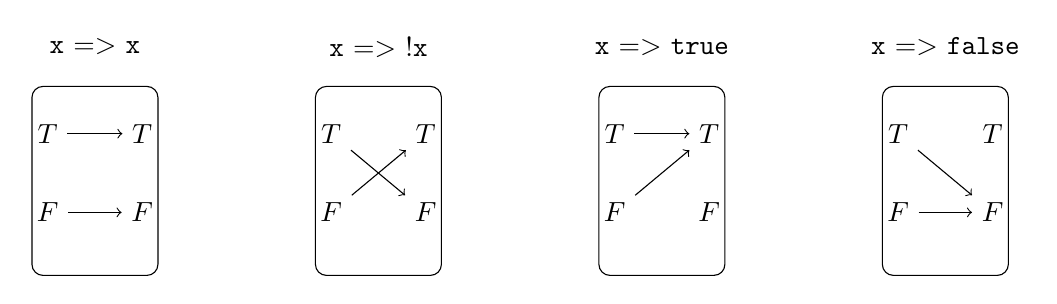
\begin{tikzpicture}
  % panel 1: x => x
  \node at (-5.4,1.6) {$\mathtt{x\ {=}{>}\ x}$};
  \draw[rounded corners] (-6.2,1.1) rectangle (-4.6,-1.3);
  \node (A1T) at (-6,0.5) {$T$};
  \node (A1F) at (-6,-0.5) {$F$};
  \node (B1T) at (-4.8,0.5) {$T$};
  \node (B1F) at (-4.8,-0.5) {$F$};
  \draw[->] (A1T) -- (B1T);
  \draw[->] (A1F) -- (B1F);

  % panel 2: x => !x
  \node at (-1.8,1.6) {$\mathtt{x\ {=}{>}\ !x}$};
  \draw[rounded corners] (-2.6,1.1) rectangle (-1,-1.3);
  \node (A2T) at (-2.4,0.5) {$T$};
  \node (A2F) at (-2.4,-0.5) {$F$};
  \node (B2T) at (-1.2,0.5) {$T$};
  \node (B2F) at (-1.2,-0.5) {$F$};
  \draw[->] (A2T) -- (B2F);
  \draw[->] (A2F) -- (B2T);

  % panel 3: x => true
  \node at (1.8,1.6) {$\mathtt{x\ {=}{>}\ true}$};
  \draw[rounded corners] (1,1.1) rectangle (2.6,-1.3);
  \node (A3T) at (1.2,0.5) {$T$};
  \node (A3F) at (1.2,-0.5) {$F$};
  \node (B3T) at (2.4,0.5) {$T$};
  \node (B3F) at (2.4,-0.5) {$F$};
  \draw[->] (A3T) -- (B3T);
  \draw[->] (A3F) -- (B3T);

  % panel 4: x => false
  \node at (5.4,1.6) {$\mathtt{x\ {=}{>}\ false}$};
  \draw[rounded corners] (4.6,1.1) rectangle (6.2,-1.3);
  \node (A4T) at (4.8,0.5) {$T$};
  \node (A4F) at (4.8,-0.5) {$F$};
  \node (B4T) at (6,0.5) {$T$};
  \node (B4F) at (6,-0.5) {$F$};
  \draw[->] (A4T) -- (B4F);
  \draw[->] (A4F) -- (B4F);
\end{tikzpicture}
\end{document}
